\documentclass[12pt,a4paper]{report}

\usepackage[utf8]{inputenc}
\usepackage[romanian,english]{babel}
\renewcommand\familydefault{\sfdefault}

\usepackage[table,xcdraw]{xcolor}
\usepackage[margin=2.54cm]{geometry}
\usepackage{graphicx}

\usepackage{textcase}
\usepackage[titletoc, title]{appendix}
\usepackage{titlesec}
\titleformat{\chapter}{\large\bfseries\MakeUppercase}{\thechapter}{2ex}{}[\vspace*{-1.5cm}]
\titleformat*{\section}{\large\bfseries}
\titleformat*{\subsection}{\large\bfseries}
\titleformat*{\subsubsection}{\large\bfseries}

\usepackage{float}
\usepackage{microtype}
\usepackage{nicefrac}
\usepackage{amsfonts}
\usepackage{url}
\usepackage{multirow}
\usepackage{amssymb,amsmath,amsfonts,amsthm,bm}
\usepackage{tabularx}
\usepackage{listings}

\definecolor{codegray}{rgb}{0.5,0.5,0.5}
\definecolor{backcolour}{rgb}{0.95,0.95,0.92}

\lstdefinestyle{mystyle}{
    backgroundcolor=\color{backcolour},
    numberstyle=\tiny\color{codegray},
    basicstyle=\ttfamily\footnotesize,
    breakatwhitespace=false,
    breaklines=true,
    captionpos=b,
    keepspaces=true,
    numbers=left,
    numbersep=5pt,
    showspaces=false,
    showstringspaces=false,
    showtabs=false,
    tabsize=2
}
\lstset{style=mystyle,
  literate={ă}{{\u{a}}}1 {â}{{\^{a}}}1 {î}{{\^{i}}}1 {ș}{{\c{s}}}1 {ț}{{\c{t}}}1
           {Ă}{{\u{A}}}1 {Â}{{\^{A}}}1 {Î}{{\^{I}}}1 {Ș}{{\c{S}}}1 {Ț}{{\c{T}}}1
}

\usepackage{chngcntr}
\counterwithout{figure}{chapter}
\counterwithout{table}{chapter}
\counterwithout{equation}{chapter}

\usepackage{booktabs}
\usepackage[bookmarks,unicode,hidelinks]{hyperref}

\usepackage{array}
\usepackage{paralist}
\usepackage{verbatim}
\usepackage{subfig}
\usepackage{enumitem}
\setlist{noitemsep}

%%% HEADERS & FOOTERS
\usepackage{fancyhdr}
\pagestyle{empty}
\renewcommand{\headrulewidth}{0pt}
\renewcommand{\footrulewidth}{0pt}
\lhead{}\chead{}\rhead{}
\lfoot{}\cfoot{\thepage}\rfoot{}

\newcommand{\HeaderLineSpace}{-0.25cm}
\newcommand{\UniTextEN}{UNIVERSITY POLITEHNICA OF BUCHAREST \\[\HeaderLineSpace]
FACULTY OF AUTOMATIC CONTROL AND COMPUTERS \\[\HeaderLineSpace]
COMPUTER SCIENCE AND ENGINEERING DEPARTMENT\\}
\newcommand{\DiplomaEN}{Scientific Report \#4}
\newcommand{\AdvisorEN}{Scientific advisors:}
\newcommand{\BucEN}{BUCHAREST}

\newcommand{\frontPage}[6]{
\begin{titlepage}
\begin{center}
{\Large #1}
\vspace{50pt}
\begin{tabular}{p{6cm}p{4cm}}

\includegraphics[scale=0.8]{figures/upb-logo.jpg} &
	
\includegraphics[scale=0.5,trim={14cm 11cm 2cm 5cm},clip=true]{figures/cs-logo.pdf}
\end{tabular}

\vspace{105pt}
{\Huge #2}\\
\vspace{40pt}
{\Large #3}\\ \vspace{0pt}
{\Large #4}\\
\vspace{40pt}
{\LARGE \Name}\\
\end{center}
\vspace{60pt}
\begin{tabular*}{\textwidth}{@{\extracolsep{\fill}}p{6cm}r}
&{\large\textbf{#5}}\vspace{10pt}\\
&{\large \AdvisorA}\\
&{\large \AdvisorB}\\
&{\large \AdvisorC}
\end{tabular*}
\vspace{20pt}
\begin{center}
{\large\textbf{#6}}\\
\vspace{0pt}
{\normalsize \Year}
\end{center}
\end{titlepage}
}

\newcommand{\frontPageEN}{\frontPage{\UniTextEN}{\DiplomaEN}{\ProjectTitleEN}{\ProjectSubtitleEN}{\AdvisorEN}{\BucEN}}

\linespread{1.15}
\setlength\parindent{0pt}
\setlength\parskip{.28cm}

\newcommand{\AbstractPage}{
\begin{titlepage}
\textbf{\large ABSTRACT}\par
\AbstractEN \vfill
\end{titlepage}
}

\tolerance=1
\emergencystretch=\maxdimen
\hyphenpenalty=10000
\hbadness=10000
\sloppy

%%%%%%%%%%%%%%%%%%%%%%%%%%%%%%%%%%%%%%%%%%%%%%%%%%

\newcommand{\ProjectTitleEN}{Cross-Lingual and Large Language Model Approaches to Aspect-Based Sentiment Analysis}
\newcommand{\ProjectSubtitleEN}{Master Program IISC}
\newcommand{\Name}{Victor-Iulian Istrătescu}
\newcommand{\AdvisorA}{Assoc.Prof.PhD.Habil.Engr. Elena-Simona Apostol}
\newcommand{\AdvisorB}{Assoc.Prof.PhD.Habil.Engr. Cirpian-Octavia Truică}
\newcommand{\AdvisorC}{PhD.Stud.Engr. Ana-Maria Luisa Mocanu}
\newcommand{\Year}{2026}

\title{Raport de cercetare}
\author{\Name}
\date{\Year}

\newcommand{\AbstractEN}{This report extends our previous work on out-of-domain generalisation in generative ABSA by investigating two complementary directions: the use of large language models in few-shot settings and the application of fine-tuned models to Romanian, a language with limited ABSA resources. We evaluate three LLMs (Gemma2 27B, Qwen2.5 32B, Command-R) in zero-shot and six-shot configurations on both the English SemEval ASTE benchmark and a Romanian aspect-based sentiment dataset (eMAG phone reviews). We compare their performance against fine-tuned models of varying sizes and language specialisation: FLAN-T5-base (250M, English-centric), XLM-R-base (278M, multilingual), and two Romanian-specific BERT models (RoBERT-base 114M, bert-base-romanian-cased 110M). Our findings indicate that fine-tuned models at 110--278M parameters consistently match or outperform 27--32B parameter LLMs in few-shot settings on both English extraction tasks and Romanian classification tasks. Among the Romanian models, we observe that monolingual pre-training provides an advantage over multilingual models for this specific task.}

\begin{document}

\frontPageEN

\begingroup
\linespread{1}
\tableofcontents
\endgroup

\AbstractPage


\chapter{Implementation}\label{ch:implementation}

This chapter covers the data used in our experiments (Section~\ref{sec:datasets}), the LLM inference setup 
together with retrieval strategy for few-shot prompting (Section~\ref{sec:llm-inference}), 
the fine-tuning strategies of the three discriminative models (Section~\ref{sec:classifier-models}) 
and the Flan T5 model (Section~\ref{sec:gen-model-ro}) for the romanian language experiments, as well as the 
additions to the experimental pipeline as a whole (Section~\ref{sec:pipeline}).

\section{Datasets}\label{sec:datasets}

For English, we use the same SemEval ASTE setup as the previous report: train on Rest14 (1266 sentences), test on Rest14 (in-domain), Rest15, Rest16, and Laptop14 (out-of-domain).

For Romanian, we use a dataset of phone reviews from eMAG. The annotation process involved GPT-4: given a review sentence, GPT-4 assigned polarity (positive/negative/neutral) and category labels from a predefined 11-class taxonomy (experience, durability, performance, battery, price\_quality, design, camera, audio, software, brand, service). A human reviewer then verified and corrected the labels. The test set was annotated separately using the same process. Unlike SemEval ASTE, this dataset does not include aspect or opinion span annotations — only polarity and category.

The training set has 27,630 sentences with 90,778 (polarity, category) labels (about 3.3 per sentence on average). Vocabulary size is 65,188 unique words. Sentences are long compared to SemEval: mean 43.5 words, median 23, maximum 309. In T5 subword tokens: mean 73.6, median 39, P95 = 266. The test set has 3,093 sentences with 9,478 labels.

Polarity is imbalanced: 72.4\% positive, 22.6\% negative, 5.0\% neutral in training. The test set has more neutral examples (8.7\%). Figure~\ref{fig:r4-polarity} shows the polarity distribution, Figure~\ref{fig:r4-categories} shows the category distribution (experience is most common at 25.7\%), and Figure~\ref{fig:r4-sentlen} shows sentence length histograms.

\begin{figure}[H]
\centering
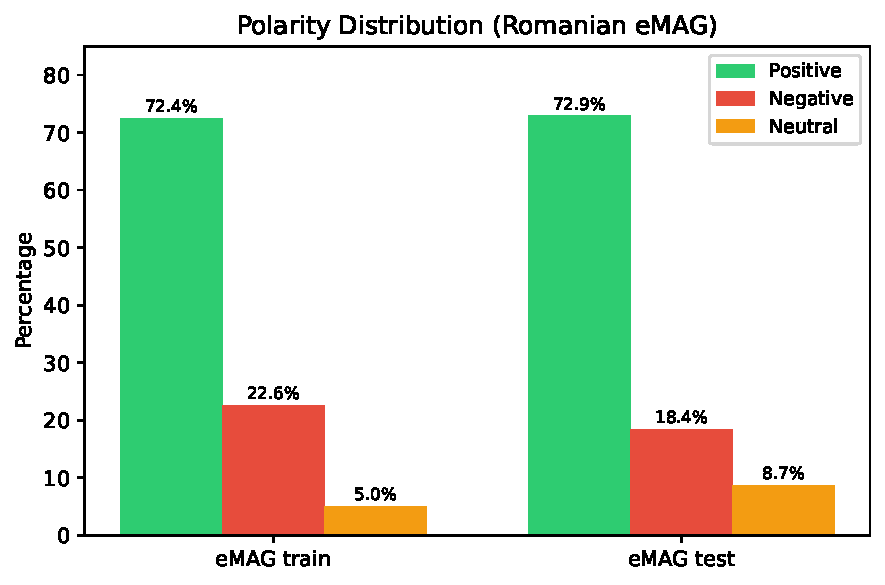
\includegraphics[width=0.7\textwidth]{figures/r4_polarity_distribution.pdf}
\caption{Polarity distribution in the Romanian eMAG training and test sets.}
\label{fig:r4-polarity}
\end{figure}

\begin{figure}[H]
\centering
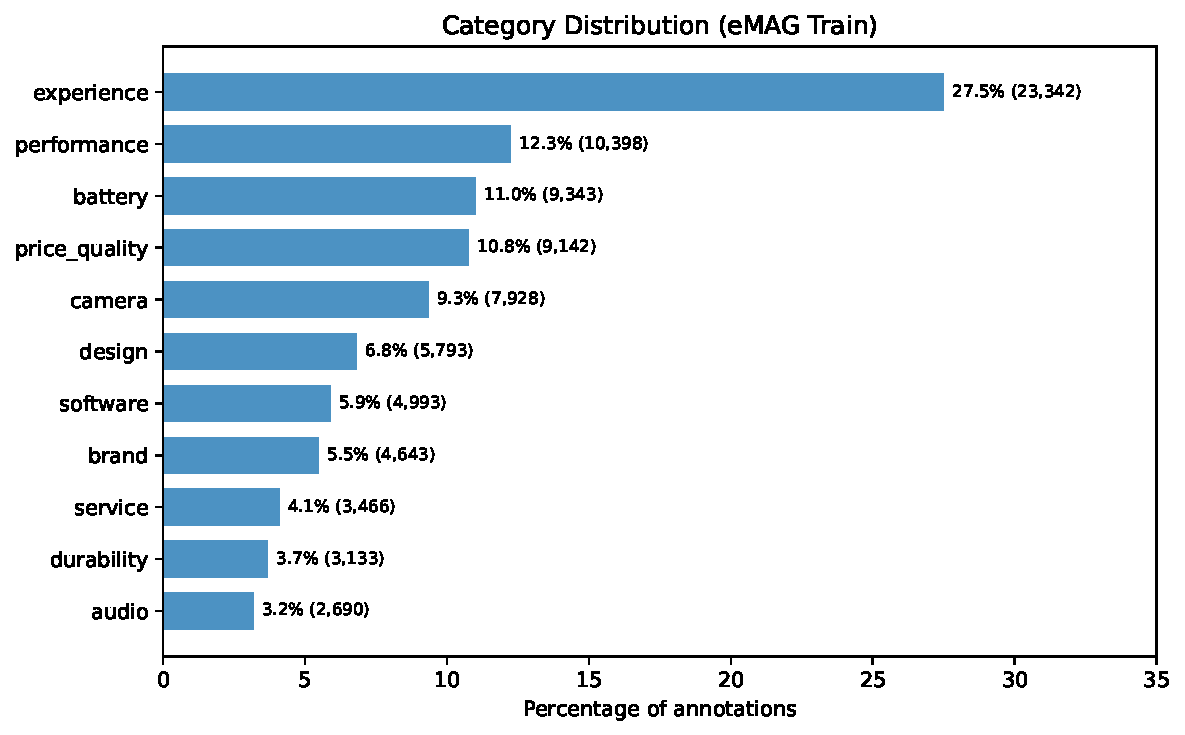
\includegraphics[width=0.85\textwidth]{figures/r4_category_distribution.pdf}
\caption{Category distribution in the Romanian eMAG training set (11 classes).}
\label{fig:r4-categories}
\end{figure}

\begin{figure}[H]
\centering
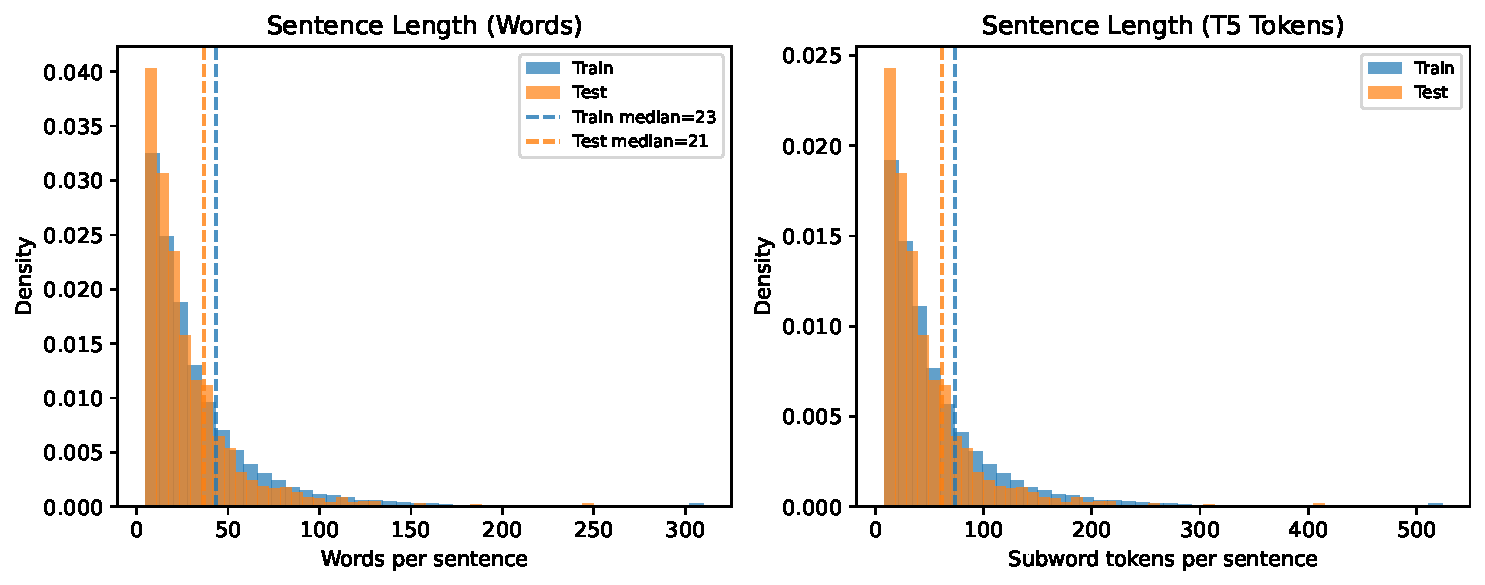
\includegraphics[width=0.95\textwidth]{figures/r4_sentence_length_histogram.pdf}
\caption{Sentence length distributions for the Romanian eMAG dataset at word and subword token level.}
\label{fig:r4-sentlen}
\end{figure}

\section{LLM Inference}\label{sec:llm-inference}

We evaluate three 4-bit quantised LLMs (Gemma2 27B, Qwen2.5 32B, Command-R), using the ollama server, in both 0-shot
and few-shot setups. In the few-shot setting we provide the model with six examples retrieved from the corresponding training set of
the data used. The examples are extracted using a hybrid approach, combining the BM25~\cite{robertson2009bm25} and
SimCSE~\cite{gao2021simcse} methods. Each technique is used to select half of the examples. We hope this will result in an optimal
balance of lexical and semantic similarity between the test sentence and examples.

The outputs were evaluated in the same fashion as for the other models: only exact predictions count as correct.

\section{Classifier Models}\label{sec:classifier-models}

For RoBERT, bert-base-romanian-cased, and XLM-R we load the pre-trained encoder and add a two-layer MLP classification head on top of the \texttt{[CLS]} representation. Since each sentence can have multiple (category, polarity) annotations, we frame the task as multi-label classification over all 33 possible category×polarity combinations (11 categories × 3 polarities) and train with binary cross-entropy loss over all label positions, applying a 0.5 threshold to the sigmoid outputs at inference time to determine which labels are present.

The training hyperparameters are fairly standard and are shared across models. 
We use a learning rate of $2 \times 10^{-5}$, weight decay 0.01, warmup ratio 0.06, batch size 16, gradient 
clipping 1.0, and bf16 mixed precision. Training runs for up to 8 epochs with early stopping at patience 3 (judged
based on validation F1 score). Because the romanian dataset does not include a dedicated validation set
we randomly selected 10\% of training data for this purpose.

\section{Generative Model (Romanian)}\label{sec:gen-model-ro}

We fine-tune FLAN-T5-base on the Romanian training set using natural-language output templates, 
following the same approach as our English experiments. We use a learning rate of $3 \times 10^{-4}$ 
with a cosine schedule, 12 epochs, and an effective batch size of 32. The model generates Romanian 
text in a fixed template format which we then parse into polarity-category pairs.

\section{Data Pipeline}\label{sec:pipeline}

Figure~\ref{fig:pipeline-r4} shows the complete training and evaluation pipeline. This architecture builds on
what was presented in the previous report, the changes being exclusively additive. Two new paths have been added,
besides the generative one: the Classifier Path, which exposes the three BERT-based models and the LLM Inference Path which adds another three models to the setup. 
For each of the new paths, we added specific data loaders, parsers and evaluation metrics.

\begin{figure}[p]
\centering
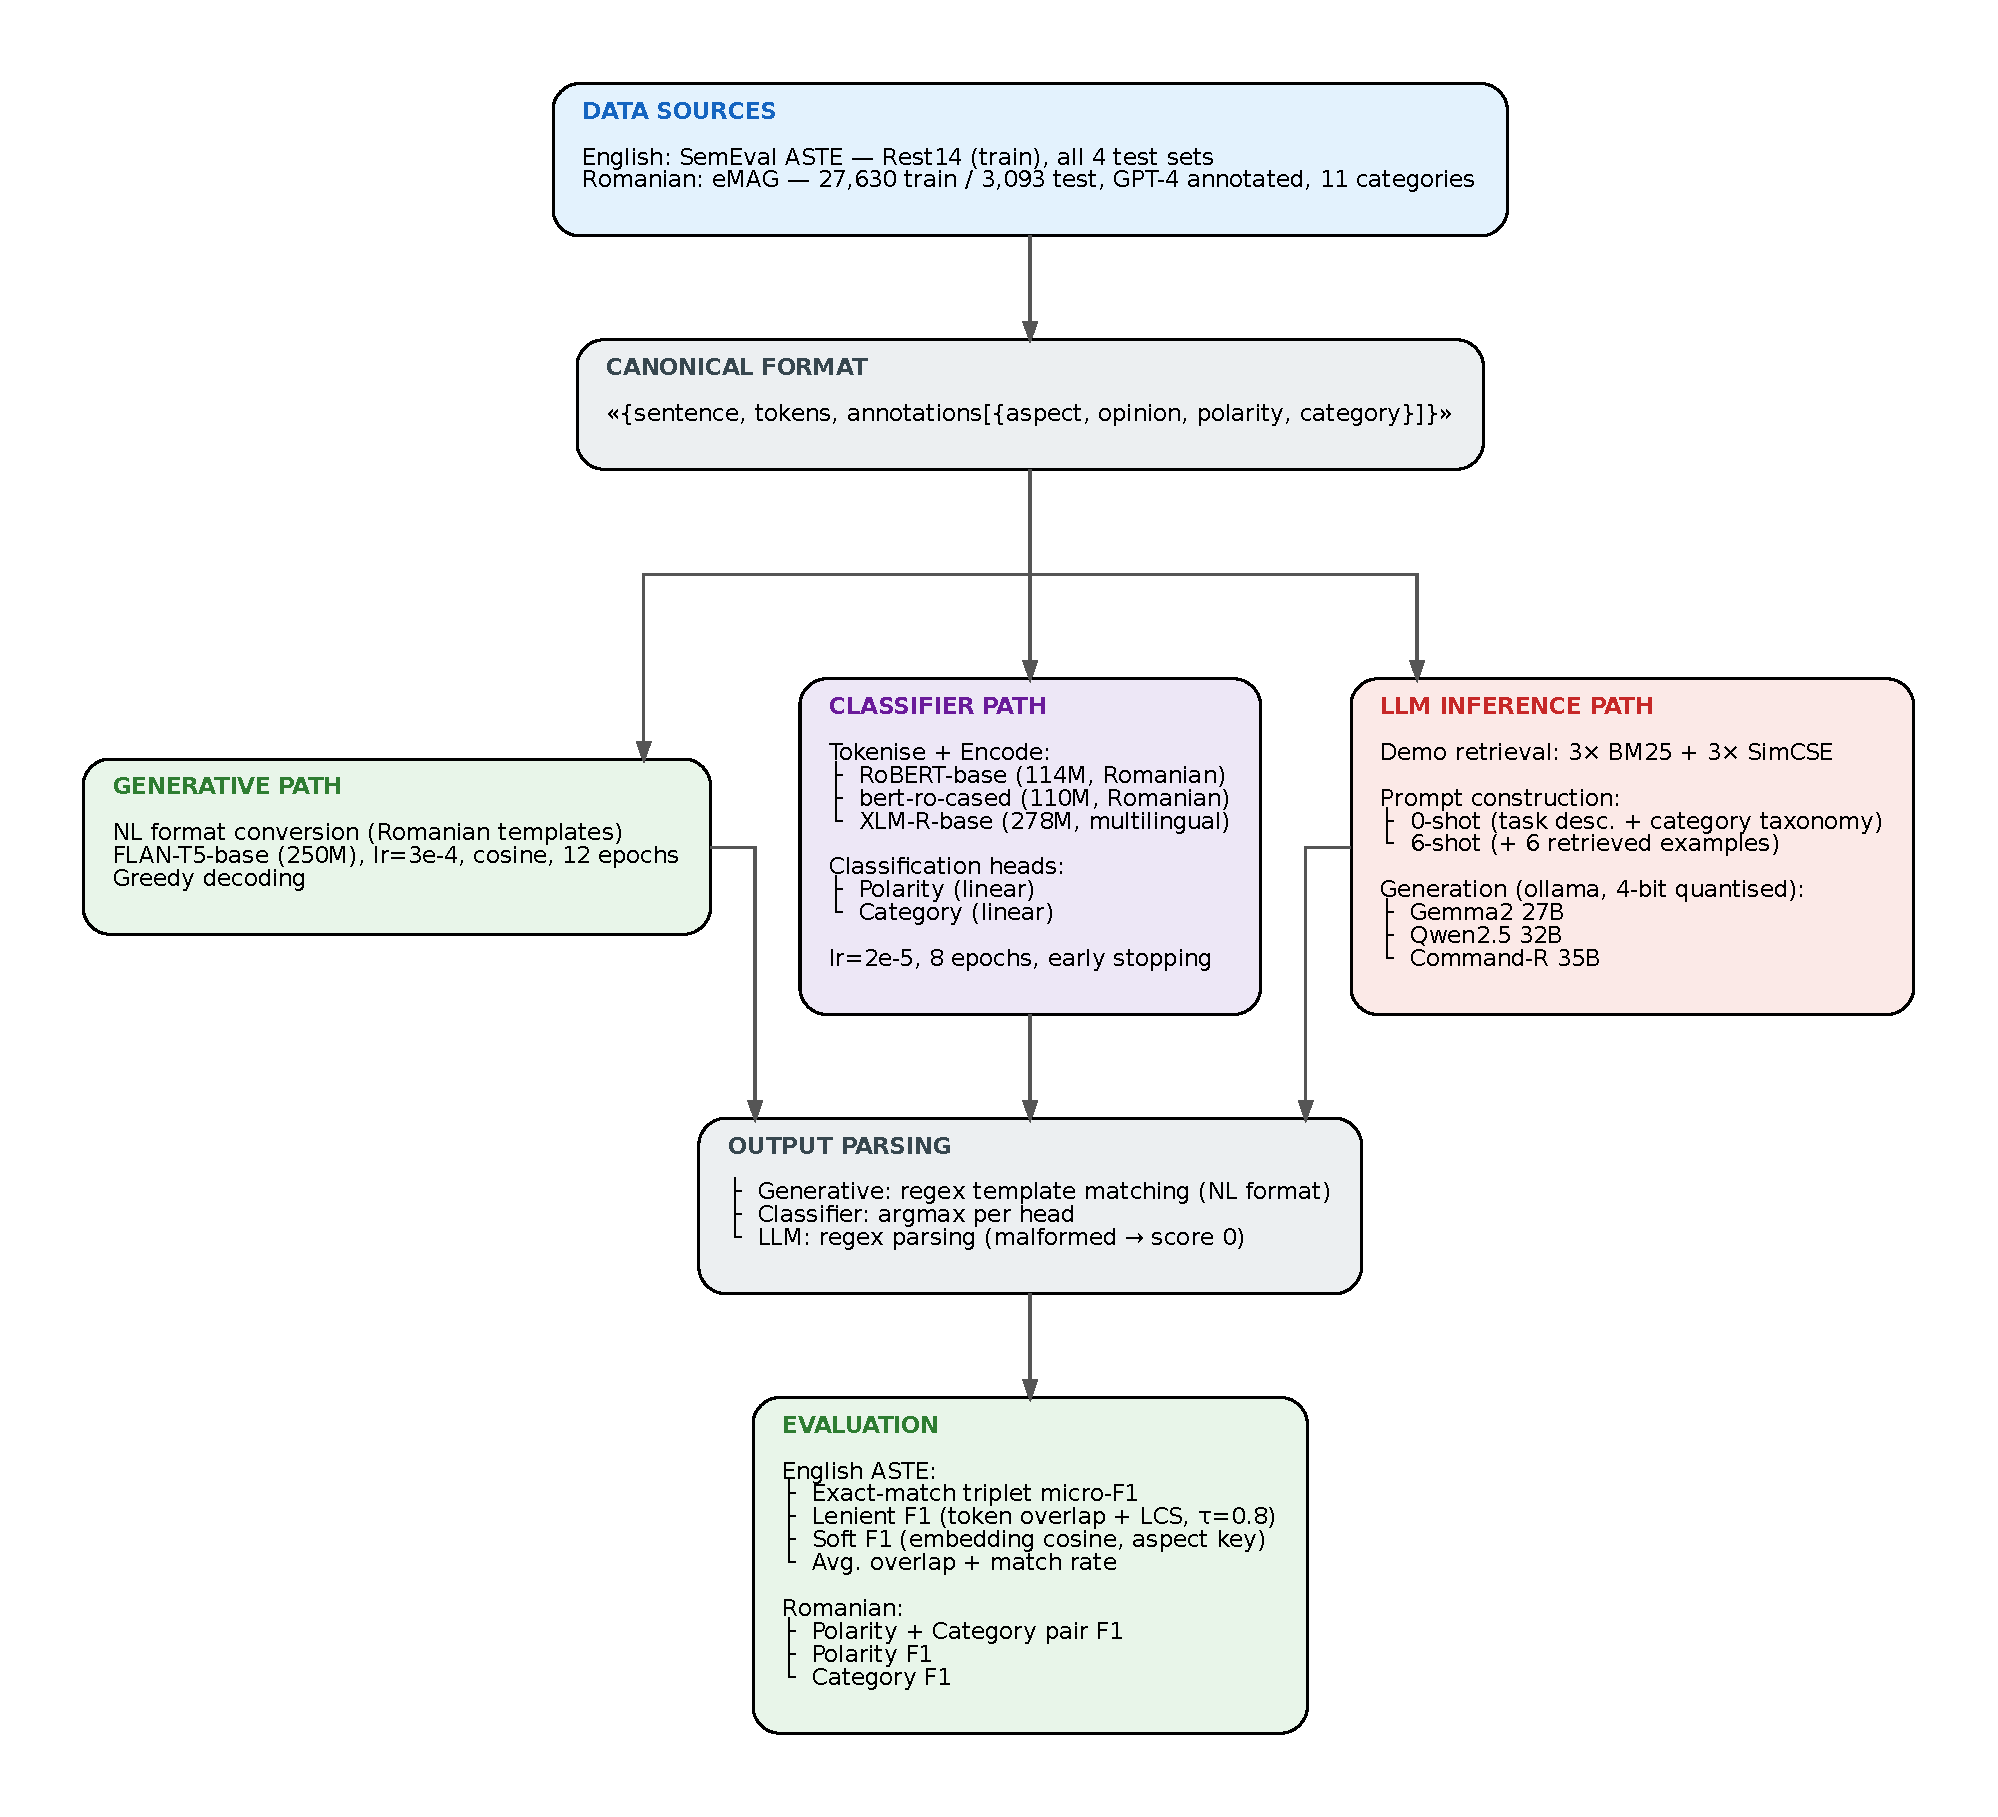
\includegraphics[width=\textwidth, height=0.88\textheight, keepaspectratio]{figures/pipeline_report4.pdf}
\caption{Evaluation pipeline showing the three parallel model paths: generative (FLAN-T5), classifier (BERT variants), and LLM inference.}
\label{fig:pipeline-r4}
\end{figure}

\chapter{Experimental Results}\label{ch:results}

This chapter presents results from both evaluation paths: LLMs on the English SemEval ASTE benchmark 
(Section~\ref{sec:llm-english}), LLMs and fine-tuned models on Romanian ABSA (Section~\ref{sec:llm-romanian}), 
followed by a discussion of monolingual versus multilingual model performance (Section~\ref{sec:mono-vs-multi}) 
and the implications of annotation quality for interpreting these results (Section~\ref{sec:annotation}).

\section{LLMs on English ASTE}\label{sec:llm-english}

\begin{table}[H]
\centering
\caption{Cross-method comparison on SemEval ASTE (triplet micro-F1). LLMs use per-dataset examples for 6-shot.}
\label{tab:llm-semeval}
\small
\begin{tabular}{@{}lrcccc@{}}
\toprule
\textbf{Method} & \textbf{Params} & \textbf{Rest14} & \textbf{Rest15} & \textbf{Rest16} & \textbf{Laptop14} \\
\midrule
\multicolumn{6}{l}{\textit{LLMs (few-shot, no fine-tuning)}} \\
\midrule
Gemma2 27B 0-shot & 27B & 0.441 & 0.418 & 0.455 & 0.275 \\
Gemma2 27B 6-shot & 27B & 0.646 & 0.592 & 0.637 & 0.410 \\
Qwen2.5 32B 0-shot & 32B & 0.535 & 0.451 & 0.556 & 0.363 \\
Qwen2.5 32B 6-shot & 32B & 0.603 & 0.527 & 0.614 & 0.370 \\
Command-R 0-shot & 35B & 0.318 & 0.256 & 0.309 & 0.206 \\
Command-R 6-shot & 35B & 0.576 & 0.499 & 0.568 & 0.373 \\
\midrule
\multicolumn{6}{l}{\textit{Fine-tuned models}} \\
\midrule
RoBERTa span & 125M & 0.544 & 0.461 & 0.560 & 0.379 \\
T5 structured & 250M & 0.693 & 0.575 & 0.640 & 0.439 \\
T5 NL baseline & 250M & \textbf{0.722} & \textbf{0.602} & \textbf{0.680} & \textbf{0.525} \\
\bottomrule
\end{tabular}
\end{table}

The fine-tuned T5 models produced the best overall results, on the SemEval data. Out of the two output formats
evaluated, the natural language format leads with an average of +0.32 ID and a much more noticeable advantage of
approximately 0.11 OOD.

Out of the three LLMs, Gemma2 with 6-shot performs best across all datasets. The advantage provided by the
few-shot setting substantial, especially for Gemma2 and Command-R, that benefit from an average increase in F1
score of 0.174 and 0. respectively. Interestingly, although in the Laptop14 few-shot evaluation, the 6 examples presented
to the models were picked from the Rest14 dataset, to simulate OOD testing, the drop in performance between
few-shot and 0-shot did not increase compared to in-domain, suggesting that the LLMs were not particularly affected
by the vocabulary shift.

Our naive fine-tuned RoBERTa baseline performs comparably to the
LLMs in 6-shot on Laptop14, falling behind with only 0.031 from Gemma2's score of 0.410. In ID setting, we observe a larger performance
gap, with results almost identical to 0-shot Qwen2.5.

\begin{figure}[H]
\centering
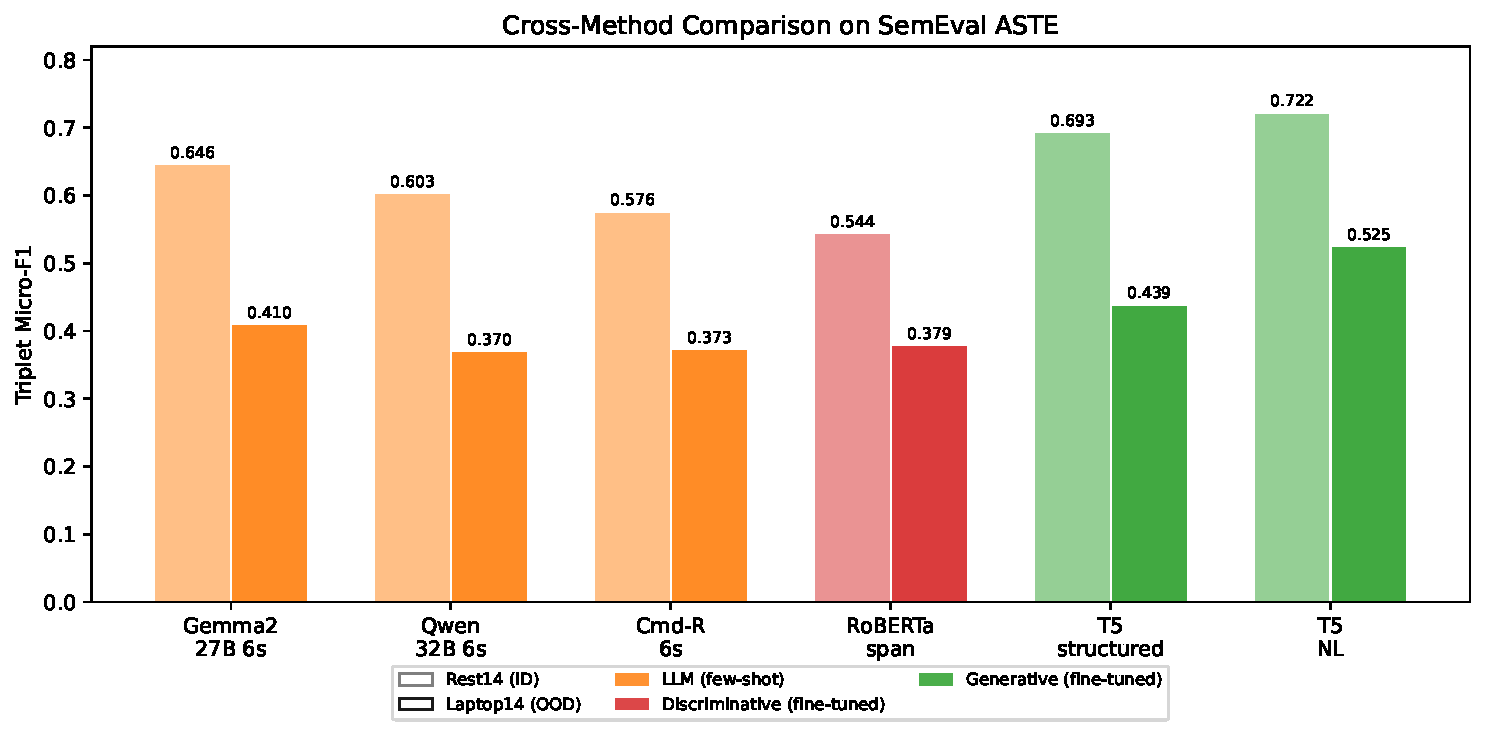
\includegraphics[width=0.95\textwidth]{figures/r4_crossmethod_english.pdf}
\caption{Cross-method comparison on SemEval ASTE: LLMs (few-shot) vs fine-tuned models, showing both in-domain (Rest14) and out-of-domain (Laptop14) performance.}
\label{fig:r4-crossmethod}
\end{figure}


\section{LLMs on Romanian ABSA}\label{sec:llm-romanian}

\begin{table}[H]
\centering
\caption{Romanian ABSA results on eMAG phone reviews. Pair F1 = polarity + category must both match.}
\label{tab:romanian}
\small
\begin{tabular}{@{}lrccc@{}}
\toprule
\textbf{Method} & \textbf{Params} & \textbf{Pair F1} & \textbf{Polarity F1} & \textbf{Category F1} \\
\midrule
\multicolumn{5}{l}{\textit{LLMs (few-shot, no fine-tuning)}} \\
\midrule
Gemma2 27B 0-shot & 27B & 0.745 & \textbf{0.888} & 0.804 \\
Gemma2 27B 6-shot & 27B & 0.758 & \textbf{0.888} & 0.826 \\
Qwen2.5 32B 0-shot & 32B & 0.621 & 0.854 & 0.689 \\
Qwen2.5 32B 6-shot & 32B & 0.740 & 0.881 & 0.807 \\
Command-R 0-shot & 35B & 0.535 & 0.766 & 0.612 \\
Command-R 6-shot & 35B & 0.750 & 0.880 & 0.821 \\
\midrule
\multicolumn{5}{l}{\textit{Fine-tuned models}} \\
\midrule
RoBERT-base (RO) & 114M & 0.792 & 0.878 & \textbf{0.862} \\
bert-base-ro-cased & 110M & 0.793 & 0.877 & 0.858 \\
XLM-R-base & 278M & \textbf{0.795} & 0.881 & 0.861 \\
FLAN-T5-base (NL) & 250M & 0.764 & 0.882 & 0.853 \\
\bottomrule
\end{tabular}
\end{table}


XLM-R-base (278M, multilingual) achieves the overall best pair F1 of 0.795, followed closely by the two monolingual 
Romanian models: bert-base-romanian-cased at 0.793 and RoBERT-base at 0.792, while FLAN-T5-base falls behind slightly. 
All fine-tuned models outperform all LLMs on pair F1 by an average of roughly 0.1.

Polarity classification alone proved to be a relatively easy for all methods, with only 0-shot Command-R scoring under 0.85. 
The bottleneck is category prediction, where LLMs score 0.61--0.83 while fine-tuned models achieve 0.85--0.86. We believe this is due to 
the taxonomy (11 classes) being specific to this dataset and not something LLMs would have encountered during 
pre-training. The 6-shot examples help LLMs learn the taxonomy, enabling a jump of roughly 0.2 in Category F1 for Command-R, but they still fall short of fine-tuned models that have seen the full training 
set.

Gemma2 stands out the most: in 0-shot it achieves 0.745 pair F1 without any task-specific data, nearly matching 
the fine-tuned FLAN-T5. Interestingly, Gemma2 is by far the most English-centric of the three, 
it's training data being primarily English~\cite{team2024gemma}. By contrast, Qwen2.5 is reported to have been
trained on more than 29 languages, including Romanian~\cite{hui2024qwen2} and Command-R on 10 major languages, although Romanian was
not included~\cite{cohere2024commandr}.

\begin{figure}[H]
\centering
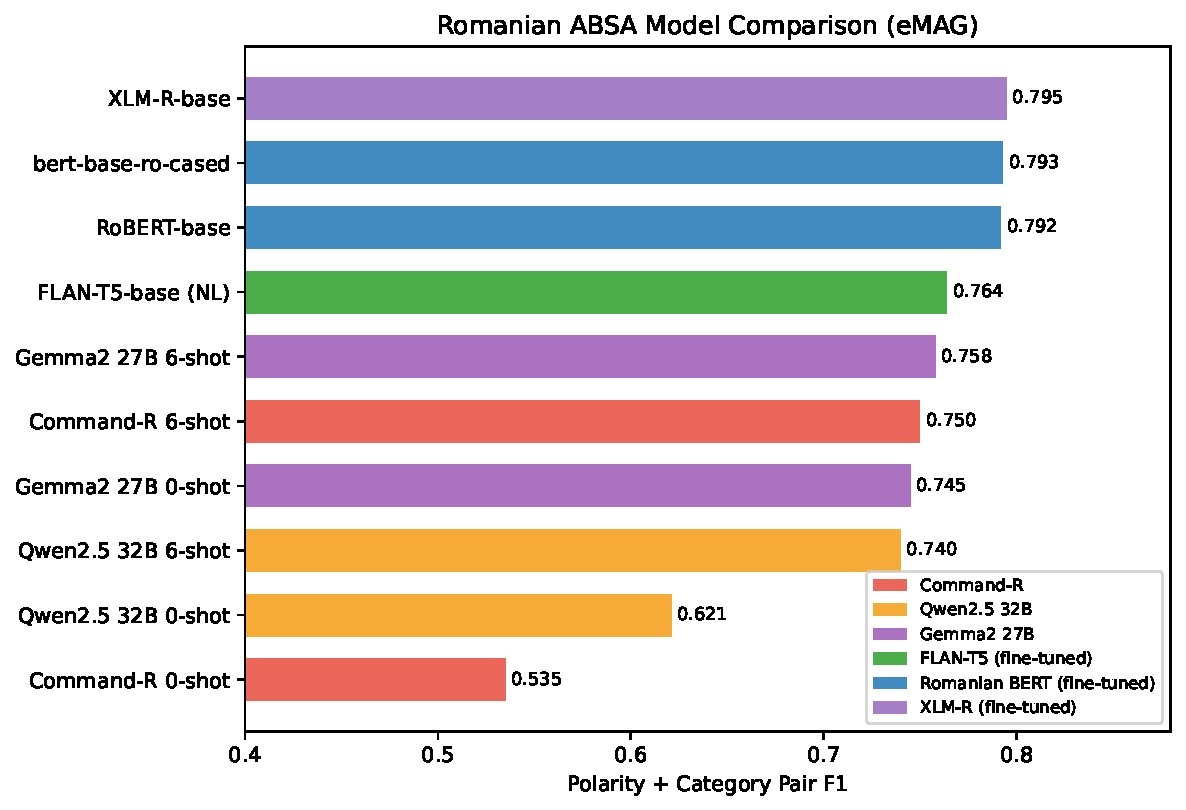
\includegraphics[width=0.85\textwidth]{figures/r4_romanian_comparison.pdf}
\caption{Romanian ABSA model comparison: all models ranked by polarity + category pair F1.}
\label{fig:r4-romanian}
\end{figure}

\begin{figure}[H]
\centering
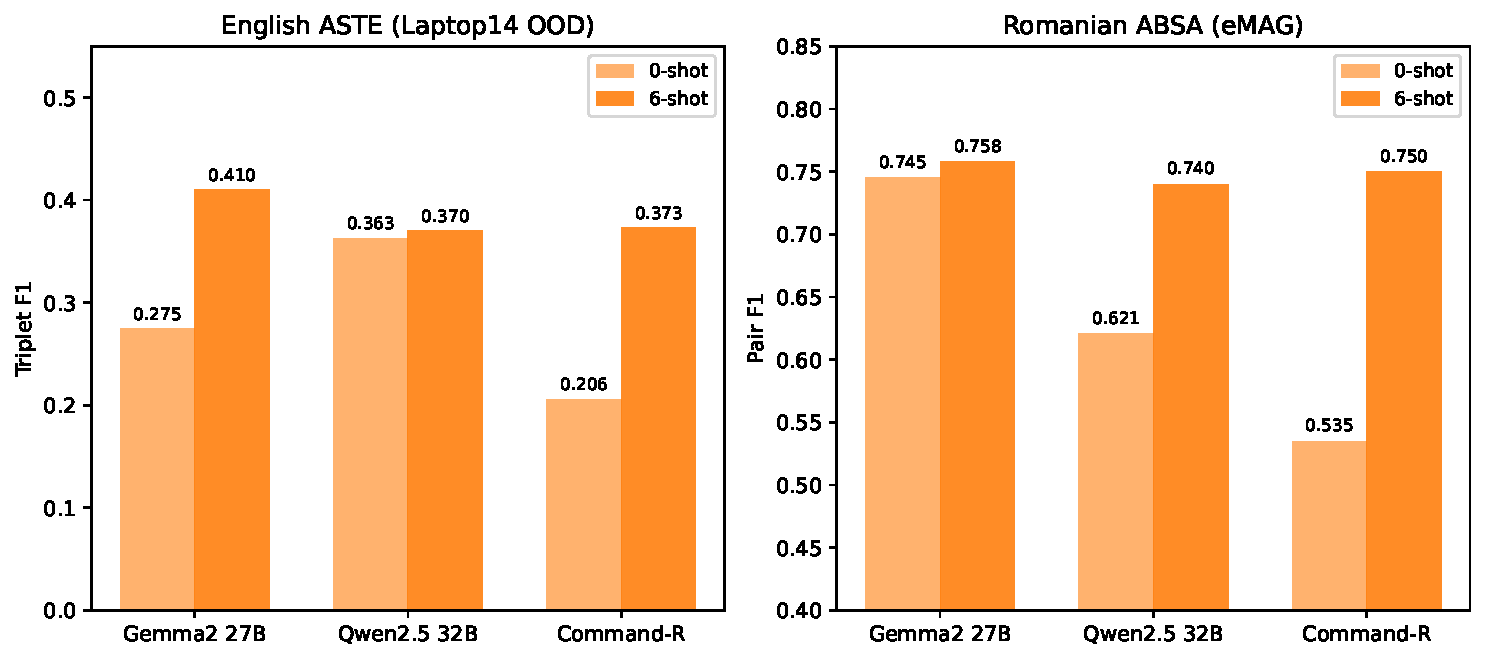
\includegraphics[width=0.95\textwidth]{figures/r4_llm_0shot_vs_6shot.pdf}
\caption{LLM performance in 0-shot vs 6-shot settings on English ASTE (left) and Romanian ABSA (right).}
\label{fig:r4-0vs6}
\end{figure}

\section{Discussion: Monolingual vs Multilingual Models}\label{sec:mono-vs-multi}

The Romanian results allow a comparison across the language specialisation spectrum. 
RoBERT-base (114M, Romanian-only) and bert-base-romanian-cased (110M, Romanian-only) achieve 0.792 and 0.793 
pair F1 respectively, XLM-R-base (278M, 100 languages) reaches 0.795, FLAN-T5-base (250M, English 
instruction-tuned) obtains 0.764, and the LLMs range from 0.740 (Qwen2.5 32B, 6-shot) to 0.758 (Gemma2 
27B, 6-shot). The monolingual Romanian models, despite being 2.5$\times$ smaller than XLM-R, perform within 
0.3 F1 points of it.

Masala et al.~\cite{masala2020robert} and Dumitrescu et al.~\cite{dumitrescu2020birth} observed the 
same pattern when they introduced their respective Romanian models, finding that on POS tagging and NER, 
monolingual pre-training on dedicated Romanian corpora matched or approached larger multilingual alternatives. 
Similar findings have been reported for other languages. Velankar et al.~\cite{velankar2022mono} showed that 
monolingual Marathi BERT outperformed XLM-RoBERTa on five downstream tasks despite being substantially 
smaller, and Hasan et al.~\cite{tanvir2023bangla} found that monolingual transformers exceeded multilingual 
models on Bangla sentiment analysis even in few-shot scenarios. Our results on Romanian data confirm what
the studies suggest, that a dedicated monolingual model is likely to match or exceed a larger multilingual one on downstream tasks in that 
language, provided sufficient monolingual pre-training data exists.

Conneau et al.~\cite{conneau2020unsupervised} acknowledged this trade-off when introducing XLM-R, and 
subsequent work has termed it the ``curse of multilinguality''~\cite{chang2023multilinguality, 
pfeiffer2024breaking}. As a fixed-capacity model covers more languages, per-language performance decreases 
because the parameters must simultaneously encode the structure of all languages. 
Bérard et al.~\cite{berard2026capacity} confirmed this empirically, showing that multilingual language models 
consistently underperform monolingual counterparts due to capacity constraints. XLM-R-base distributes 
its 278M parameters across 100 languages, whereas RoBERT-base dedicates all 114M to Romanian, having been 
trained on 12GB of exclusively Romanian text. Per-parameter efficiency for Romanian is therefore much higher 
in the monolingual model. That XLM-R still edges ahead in our results (0.795 vs 0.792--0.793) may reflect 
cross-lingual transfer, as XLM-R has encountered sentiment-related patterns across many languages during 
pre-training, and some of these transfer to Romanian even without explicit supervision.

From a practical standpoint, the monolingual models offer the same performance as XLM-R at lower computational 
cost, being faster to fine-tune and requiring less memory at inference, which matters for deployment when 
target-language fine-tuning data is available and the additional capacity of a multilingual model provides 
no benefit.

FLAN-T5-base trails by 3 points despite being a 250M model, which is was expected given that it is an 
English-centric generative model performing a classification task in a language it was not primarily trained 
on. The encoder-based classifiers have a natural architectural advantage here, as they produce a single 
representation that feeds directly into classification heads, while the generative model must produce the 
correct output token by token. Although, the fact that FLAN-T5 
still reaches 0.764 and outperforms all LLMs shows that even modest fine-tuning on target-language data 
compensates for a mismatch between the model's pre-training language and the task language.

Interestingly, the relationship between language coverage and performance appears to reverse in the case
of our LLM experiments on Romanian data. 
Gemma2, the most English-centric of the three (trained on 13 trillion tokens of primarily English web 
data and officially described as ``available in English''~\cite{team2024gemma}), outperforms both Qwen2.5 
(29+ languages including Romanian~\cite{hui2024qwen2}) and Command-R (10 languages~\cite{cohere2024commandr}) 
on Romanian text. Kapo\v{c}i\={u}t\.{e}-Dzikien\.{e} et al.~\cite{kapociute2025baltic} observed a similar 
pattern when evaluating open-weight LLMs without fine-tuning on Baltic languages, where Gemma~2 performed 
close to top commercial models while explicitly multilingual LLMs struggled. In our case, the explanation 
likely lies in the task structure itself. The system prompt, category labels, and polarity names are all 
in English; only the review text is in Romanian. Recent work has shown that English-dominant LLMs convert 
non-English input into English-like internal representations in their early layers and perform reasoning 
in an English-aligned concept space before routing back to the target language in the final 
layers~\cite{wendler2024llamas, zhao2024multilingualism, schut2025multilingual}. Since our task requires 
no non-English output, this final routing step is unnecessary, and a model that concentrates all its 
capacity on English might have stronger representations precisely where the task demands them. 
The multilingual training of Qwen2.5 and Command-R seems to provide no advantage here because both the 
reasoning and the output are conducted in English regardless of the input language.


\section{Discussion: Annotation Quality and Performance Ceiling}\label{sec:annotation}

Hu and Liu~\cite{hu2004mining}, in their foundational work on opinion mining, observed that identifying what constitutes an opinion versus a factual statement is inherently subjective and context-dependent. This subjectivity propagates to annotation: Miñarro-Giménez et al.~\cite{minarro2018qualitative} found that even trained annotators show non-trivial disagreement on structured clinical text labelling tasks, with inconsistencies that cannot be eliminated through guidelines alone. The degree of annotator agreement therefore sets an upper bound on achievable model performance when evaluating against a single gold standard.

The SemEval ABSA datasets~\cite{pontiki2014semeval} are no exception. The annotation guidelines leave room for interpretation in cases involving implicit sentiment, pragmatic inference, and debatable polarity. Our error analysis on Laptop14 (detailed in the previous report) surfaced several recurring patterns where the model prediction is arguably as defensible as the gold label: ``I needed a laptop with big storage'' is annotated [storage, big, neutral] because the desire context is treated as non-opinionated, but the model predicts positive since ``big'' carries positive valence in most training examples; ``There is no HDMI receptacle'' receives a neutral label under a strict reading of the guidelines (no explicit opinion word), but the model predicts negative, which is how most readers would interpret a complaint about a missing feature; hypotheticals like ``a spice rub might have overwhelmed'' are annotated as negative opinions even though the reviewer is only presenting a hypothetical situation. Based on this analysis, we estimate that 5--10\% of Laptop14 annotations involve genuinely ambiguous polarity.

These difficult cases require pragmatic reasoning about speaker intent, speech acts, or counterfactual constructions. Li et al.~\cite{li2021implicit} showed that neural language models do develop implicit representations of entity states from text alone, but noted that these representations are incomplete. More recently, Sun et al.~\cite{sun2025implicit} argued that text embedding research remains narrowly focused on surface-level semantics rather than the implicit meaning needed for pragmatic inference. Our models, trained on surface-level aspect-opinion-polarity annotations, predictably struggle with cases where the correct label depends on understanding what the reviewer meant rather than what they literally said.

The Romanian dataset introduces additional concerns. The training data was annotated with GPT-4 assistance (polarity and category labels generated by GPT-4, then reviewed by humans), and Aldeen et al.~\cite{aldeen2023chatgpt} found that while LLM-generated annotations achieve competitive quality for straightforward sentiment classification, human annotators consistently outperform on tasks requiring nuanced contextual judgement. Category assignment is probably the most annotation-sensitive component in our setup: the boundary between ``experience'' and ``performance'', or ``design'' and ``durability'', requires domain familiarity that GPT-4 may resolve differently from a human annotator who knows Romanian consumer electronics vocabulary. There is also an inherent circularity when we train models on LLM-annotated data and then evaluate LLMs on test data from the same annotation pipeline. We mitigate this by using an independently annotated test set, but biases in the training set still propagate to all fine-tuned models. Gemma2 27B achieves approximately 0.75 pair F1 on Romanian in 0-shot, and GPT-4 is likely somewhat better but not dramatically so on this specific task, so the training data quality ceiling is bounded by what an imperfect annotator can produce. The proportion of ambiguous annotations in the Romanian data may be higher than in SemEval given the automated annotation pipeline, though we have not quantified it precisely.

For practical interpretation, these observations mean that reported F1 scores on both datasets should be read with appropriate caution. A portion of the gap between model performance and perfect F1 reflects genuine annotation ambiguity rather than model limitations. Importantly, this noise affects all methods equally: relative comparisons between models remain valid even if absolute scores overstate the underlying task difficulty. On the English side, the LLM evaluation on SemEval is free from annotation circularity since the test data was annotated by humans independently, so the LLMs' lower performance relative to fine-tuned models reflects genuine capability differences in structured extraction rather than annotation artefacts.



\chapter{Conclusions}\label{ch:conclusions}

\section{Summary}

This report investigated two extensions of our previous work on generative ABSA: the comparison of fine-tuned models against large language models, and the application to Romanian as a representative medium-resource language.

On English ASTE, fine-tuned FLAN-T5-base (250M parameters) outperforms all tested LLMs (27--35B parameters) in both zero-shot and six-shot settings. The gap is 11.5 F1 points on out-of-domain data (Laptop14) between our best model and the best LLM. This is consistent with findings in the literature for structured extraction tasks: task-specific fine-tuning remains more effective than in-context learning at current LLM scales.

On Romanian ABSA, fine-tuned models (XLM-R, RoBERT, bert-ro, FLAN-T5) outperform LLMs on the combined polarity+category metric. Polarity classification is easy for all methods ($\sim$0.88 F1), while category prediction is the bottleneck for LLMs, particularly in 0-shot where the specific taxonomy is unknown to the model. Monolingual Romanian models (110--114M) perform within 0.3 F1 points of the 2.5$\times$ larger multilingual XLM-R, confirming that dedicated language-specific pre-training compensates for smaller model size on downstream tasks.

\section{Limitations}

\begin{itemize}
    \item LLM quantisation: all LLMs are 4-bit quantised, which reduces performance relative to full-precision inference. Results represent a lower bound on LLM capability.
    \item Single inference run: LLM evaluations use a single run (no temperature variation or multiple sampling). Variance is not characterised.
    \item GPT-4 annotation: the training data annotation quality is bounded by GPT-4's capabilities on Romanian text, which may introduce systematic biases.
\end{itemize}

\section{Future Work}

\begin{itemize}
    \item Fine-tuning smaller LLMs (7--8B parameters) on ABSA tasks, to find the scale at which fine-tuned LLMs begin to outperform fine-tuned smaller models.
    \item Testing chain-of-thought prompting for LLMs on extraction tasks, which might help with the span boundary identification problem.
    \item Expanding Romanian ABSA evaluation to other product categories (not just phones) and to triplet extraction (ASTE) rather than just polarity+category classification.
    \item Evaluating the effect of increasing few-shot examples (12-shot, 24-shot) to determine how much demonstration data LLMs need to approach fine-tuned performance.
\end{itemize}


\chapter{Annex}\label{ch:annex}

\section{LLM Prompt Templates}\label{annex:few-shot-prompts}

\textbf{English ASTE (6-shot format):}
\begin{lstlisting}
[system]
You are an aspect-based sentiment analysis system. Given a review sentence, extract all (aspect, opinion, polarity) triplets.

Output format: one triplet per line as [aspect, opinion, polarity]
- aspect: the entity or feature being discussed (exact span from text)
- opinion: the opinion expression about the aspect (exact span from text)
- polarity: positive, negative, or neutral

If there are no triplets, output: none
Do not explain your reasoning. Only output the triplets.

[user]
Input: The price is reasonable although the service is poor .

[assistant]
[price, reasonable, positive]
[service, poor, negative]

... (Another 5 examples) ...

[user]
Input: The design and atmosphere is just as good .
\end{lstlisting}

\textbf{Romanian ABSA (6-shot format):}
\begin{lstlisting}
[system]
You are a sentiment analysis system for phone reviews written in Romanian. Given a review, extract all (category, polarity) pairs that are discussed.

Output format: one pair per line as [category, polarity]
- category: Must be one of: experience, durability, performance, battery, price_quality, design, camera, audio, software, brand, service
- polarity: Must be one of: positive, negative, neutral

Category descriptions (for reference):
  experience = overall satisfaction, durability = build quality/longevity,
  performance = speed/responsiveness, battery = battery life/charging,
  price_quality = value for money, design = appearance/form factor,
  camera = photo/video quality, audio = speakers/microphone,
  software = OS/apps/updates, brand = manufacturer reputation,
  service = delivery/customer support/warranty

If there are no pairs, output: none
Do not explain your reasoning. Only output the pairs.

[user]
Input: Nu merită. Se încălzește tare.

[assistant]
[experience, negative]
[performance, negative]
[price_quality, negative]

... (Another 5 examples) ...

[user]
Input: Super telefon pentru cei cunoscători!
\end{lstlisting}

\section{Per-Model LLM Results (English)}

\begin{table}[H]
\centering
\caption{Gemma2 27B detailed results (SemEval ASTE, triplet micro-F1).}
\small
\begin{tabular}{@{}lcccc@{}}
\toprule
\textbf{Setting} & \textbf{Rest14} & \textbf{Rest15} & \textbf{Rest16} & \textbf{Laptop14} \\
\midrule
0-shot & 0.441 & 0.418 & 0.455 & 0.275 \\
6-shot & 0.646 & 0.592 & 0.637 & 0.410 \\
\bottomrule
\end{tabular}
\end{table}

\begin{table}[H]
\centering
\caption{Qwen2.5 32B detailed results (SemEval ASTE, triplet micro-F1).}
\small
\begin{tabular}{@{}lcccc@{}}
\toprule
\textbf{Setting} & \textbf{Rest14} & \textbf{Rest15} & \textbf{Rest16} & \textbf{Laptop14} \\
\midrule
0-shot & 0.535 & 0.451 & 0.556 & 0.363 \\
6-shot & 0.603 & 0.527 & 0.614 & 0.370 \\
\bottomrule
\end{tabular}
\end{table}

\begin{table}[H]
\centering
\caption{Command-R detailed results (SemEval ASTE, triplet micro-F1).}
\small
\begin{tabular}{@{}lcccc@{}}
\toprule
\textbf{Setting} & \textbf{Rest14} & \textbf{Rest15} & \textbf{Rest16} & \textbf{Laptop14} \\
\midrule
0-shot & 0.318 & 0.256 & 0.309 & 0.206 \\
6-shot & 0.576 & 0.499 & 0.568 & 0.373 \\
\bottomrule
\end{tabular}
\end{table}


\clearpage
\addcontentsline{toc}{chapter}{Bibliography}
\bibliographystyle{ieeetr}
\bibliography{bibliography4}

\end{document}